\section{SW01}

\subsection{Getestet wird immer}
\label{subsec: Getestet wird immer}
Getestet wird immer, es bleibt nur offen:
\begin{itemize}
    \item Wann wird getestet?
    \item Wer testet?
    \item Wo werden die Test Resultate veröffentlicht?
\end{itemize}
Es lohnt sich das Testen vor der Entwicklung einzuplanen (Kosten, Zeitpunkt, Image Schaden).
Beispiele sind:
\begin{itemize}
    \item Unzureichender Last-Test für Ski-Gebiete Online Buchung
    \item Sirenentest musste wegen Systemfehler wiederholt werden 
    \item Oberflächenbehandlungsmaschine welche bereits mit ungenügenden Test geplant wurde (Funktion Düsen nicht interdisziplinär getestet, Positionsensor nicht auf voller Leistung getestet wegen Lärm)
\end{itemize}

\subsection{Die 10er Regel}

Die Abbildung \ref{fig:10er Regel} besagt, dass je weiter ein Fehler sich unentdeckt in die späteren Phasen des Werdeganges eines Produktes oder Prozesses bewegt, umso höher werden die Kosten zur Behebung dieses Fehlers~\cite{sixsigmablackbelt.de}.

\begin{figure}[H]
	\centering
	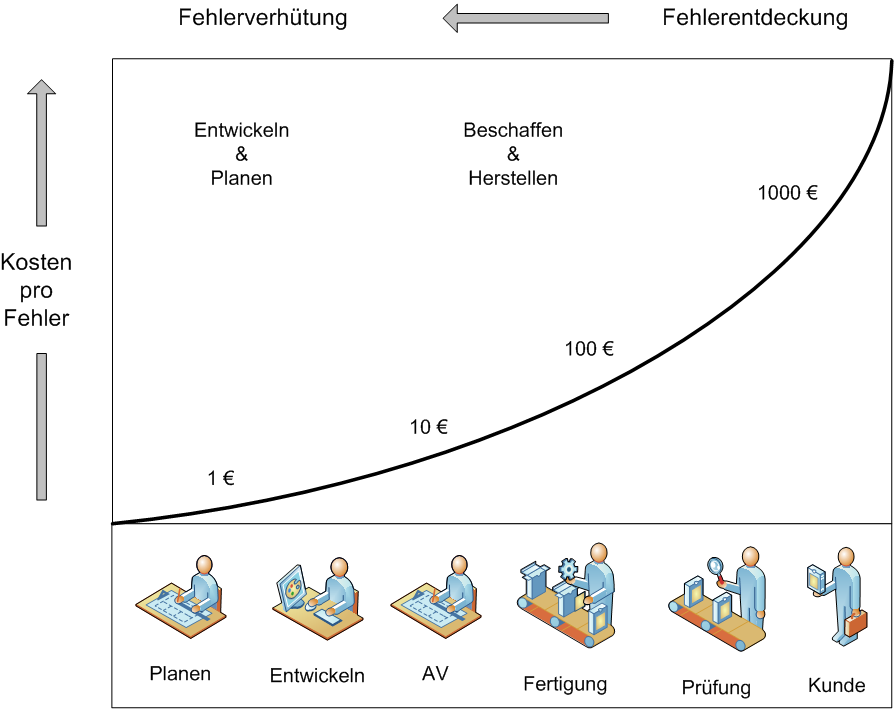
\includegraphics[width=1.0\columnwidth]{01/bilder/Fehlerkosten-10-er-Regel.png}
	\caption{Fehler-kosten der 10er Regel (rule of ten).}
	\label{fig:10er Regel}
\end{figure}

Beispiele:
\begin{itemize}
    \item Beispiele aus Unterkapitel \ref{subsec: Getestet wird immer}
    \item Heroes of Newearth Game-Entwicklung: nicht-Initialisierung einer Variable hat im 64Bit System zum Fehler geführt, welches erst beim Release durch die User bemerkt wurde. Rollback war notwendig.
\end{itemize}

\subsection{Testen bringt Nutzen}
Mehr Qualität:
\begin{itemize}
    \item wird messbar und quantifizierbar und dadurch sichtbar und verkaufbar
    \item was messbar ist, wird steuerbar
    \item kann somit gezielt gesteigert werden
\end{itemize}

Mehr Wirtschaftlichkeit:
\begin{itemize}
    \item Frühes Erkennen von Fehler ist billiger
    \item After Sales Support wird weniger (Einsparen von Kosten)
    \item Testen dokumentiert Wissen und schützt so Investitionen
    \item Ressourcen werden sinnvoll eingesetzt
\end{itemize}

Risikomanagement:
\begin{itemize}
    \item Risiken werden frühzeitig identifiziert
    \item Risiken werden aktiv gemanagt
    \item Das Eintreffen der Risiken kann vermieden werden
    \item Es wird dort getestet, wo es sinnvoll ist (in der Regel wird das getestet was man: kennt, schon immer getestet hat, gut bekannt ist)
\end{itemize}

Besserer Wettbewerbsvorteil:
\begin{itemize}
    \item keine negativ Presse
    \item hohe Reputation dank Zuverlässigkeit
    \item Erweiterbarkeit und Wartbarkeit ergeben Nachhaltigkeit
    \item swissness, Qualitätsbewusstsein
\end{itemize}


\subsection{Testqualität vs. Produktqualität}
Abbildung \ref{fig: Testqualität vs. Produktqualität} zeigt auf der X-Achse die Testqualität und auf der Y-Achse die Produktqualität~\cite{theNoserWayOfTesting}.

\begin{figure}[H]
	\centering
	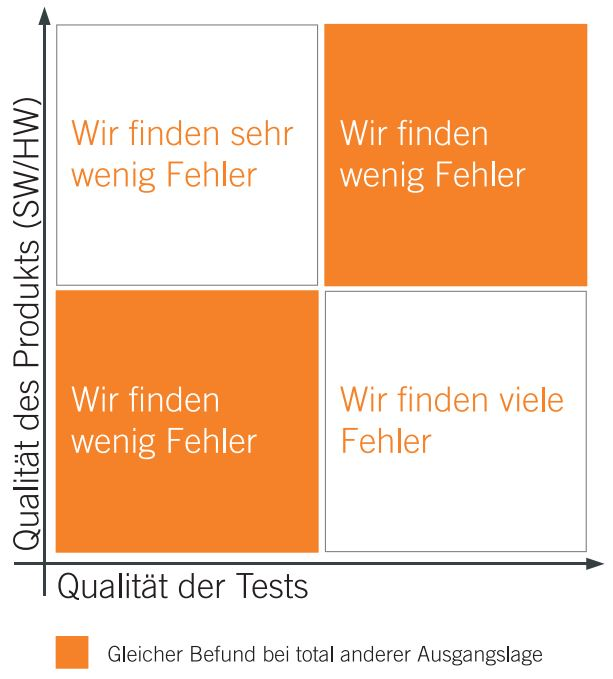
\includegraphics[width=0.6\columnwidth]{01/bilder/Testqualität vs Produktqualität.JPG}
	\caption{Testqualität gegenüber Produktqualität.}
	\label{fig: Testqualität vs. Produktqualität}
\end{figure}

Aus der Abbildung lassen sich folgende Rückschlüsse ziehen:
\begin{itemize}
    \item Der Grund fürs Testen ist es herauszufinden ob man eine gute oder schlechte Produktqualität hat.
    \item Ist die Testqualität schlecht, können keine Rückschlüsse auf die Produktqualität gewonnen werden -> Provokativ: Warum testet man dann überhaupt?
    \item Man findet sehr wenig Fehler -> gute Entwickler, schlechte Tester
    \item Man findet sehr viele Fehler -> schlechte Entwickler, gute Tester
    \item Aufpassen da man den gleichen Befund haben kann bei total unterschiedlicher Ausgangslage!
    \item Je besser das Testen, desto schlechter erscheint die Produktqualität
\end{itemize}

Das Bewerten der Fehlerzahl kann über das Messen der gefundenen Fehler im Verlaufe des Projektes bewertet werden. Abbildung \ref{fig: Fehlerkumulation über die Zeit} zeigt das Aufkumulieren der Fehler über die Zeit. Die X-Achse ist die Zeit, die Y-Achse sind alle gefundenen Fehler.

\begin{figure}[H]
	\centering
	\includegraphics[width=0.4\columnwidth]{01/bilder/Fehlerkumulation über die Zeit.JPG}
	\caption{Fehlerkumulation eines SW-Produktes über die Zeit.}
	\label{fig: Fehlerkumulation über die Zeit}
\end{figure}

Wenn der Gradient der gefundenen Fehler (rote Linien) flacher wird, ist dies ein Zeichen dafür, das mit den angewandten Methoden keine weiteren Fehler gefunden werden können. Das kann auch so interpretiert werden, das in Abbildung \ref{fig: Testqualität vs. Produktqualität} man die Qualität des Produktes gesteigert hat. Das sich die Qualität der Tests verschlechter über Zeit wird nicht angenommen.
Weitere Info's zu diesem Thema in Kapitel \textcolor{red}{Noch zu definieren - später!}.


\subsection{Anforderungen der Stakeholder}
Stellen Sie sich ein Glas / Ball vor. Ich kann ein Glas/Ball nicht testen ohne die Anforderungen der Stakeholder zu kennen. Dies beinhaltet:
\begin{itemize}
    \item Anwendungszweck
    \item Umgebung
    \item Bedürfnisse
    \item Kontext
\end{itemize}

Ein Softwaretest prüft und bewertet Software auf Erfüllung der für ihren Einsatz definierten Anforderungen und misst ihre Qualität. 
